\documentclass[aspectratio=43]{beamer}
\usepackage{luatexja-fontspec}
\usepackage{graphicx,color,multicol,verbatim,listingsutf8}
\usepackage{xcolor}
\usepackage{url,tikz}
\usepackage[symbol]{footmisc}
\usetikzlibrary{arrows.meta,calc,fit,positioning}
\usetheme{Boadilla}
\usecolortheme[RGB={140,0,0}]{structure}
\setbeamertemplate{navigation symbols}{}
\setbeamercovered{transparent}
\usefonttheme{professionalfonts}
\renewcommand\familydefault{\rmdefault}
\renewcommand{\figurename}{図\thefigure}
\renewcommand{\thefootnote}{\fnsymbol{footnote}}
\renewcommand{\thempfootnote}{\fnsymbol{mpfootnote}}
\setbeamertemplate{sections/subsections in toc}[sections numbered]
\setbeamertemplate{enumerate item}[default]
\setbeamertemplate{itemize item}[triangle]
\lstset{
        %枠外に行った時の自動改行
    breaklines = true,
        %自動改行後のインデント量(デフォルトでは20[pt])
    breakindent = 10pt,
        %標準の書体
    basicstyle = \ttfamily\small,
        %コメントの書体
    commentstyle = {\scriptsize\ttfamily \color[cmyk]{1,0.4,1,0}},
        %関数名等の色の設定
    classoffset = 0,
        %キーワード(int, ifなど)の書体
    keywordstyle = {\bfseries\ttfamily \color[cmyk]{0,1,0,0}},
        %表示する文字の書体
    stringstyle = {\ttfamily \color[rgb]{0,0,1}},
        %枠 tは上に線を記載, Tは上に二重線を記載
        %他オプション:leftline,topline,bottomline,lines,single,shadowbox
    frame = single,
        %frameまでの間隔(行番号とプログラムの間)
    framesep = 5pt,
        %行番号の位置
    numbers = left,
        %行番号の間隔
    stepnumber = 1,
        %行番号の書体
    numberstyle = \scriptsize,
        %タブの大きさ
    tabsize = 4,
        %キャプションの場所(tbならば上下両方に記載)
    captionpos = t,
    xleftmargin=1em
}
\makeatletter
\title[音声合成]{3. 音声合成}
\subtitle[]{情報学群実験第3C 3i}
\author[Group 10]{\small 門屋陽丈\and 谷保愛華\and 内藤熙人\and 成岡小雪\and 平林里菜\and 三上柊\and 溝口洸熙}
\institute[]{Group 10}
\date[2023.04.20]{April 20, 2023}
\newcommand{\showsec}{\thesection .}
\setbeamercolor{block title}{bg=black,fg=white}
\setbeamercolor{block body}{bg=gray!10,fg=black}
\begin{document}
\begin{frame}
    \titlepage
\end{frame}
\begin{frame}{お品書き}
    \begin{columns}[onlytextwidth,T]
        \begin{column}{.5\textwidth}
            \tableofcontents[sections={1-5}]
        \end{column}
        \begin{column}{.5\textwidth}
            \tableofcontents[sections={6-7}]
        \end{column}
    \end{columns}
\end{frame}
\section{初期位相・矩形波}
\begin{frame}[t]{\showsec 初期位相・矩形波}
    周波数\(f\),時刻を\(t\)に設定する.
    \begin{block}{初期位相}
        初期位相を\(\phi\)に設定する.
        \begin{align}
            y(t) & = \sin(2\pi ft+\phi)
        \end{align}
    \end{block}
    \begin{block}{矩形波のフーリエ級数展開}
        \begin{align}
            y(t) & = \sum_{k=1}^{\infty}\dfrac{1}{2k-1}\sin\big(2\pi(2k-1)ft\big)
        \end{align}
    \end{block}
\end{frame}
\section{ノコギリ波}
\begin{frame}[t]{\showsec ノコギリ波}
    \begin{figure}
        \centering
        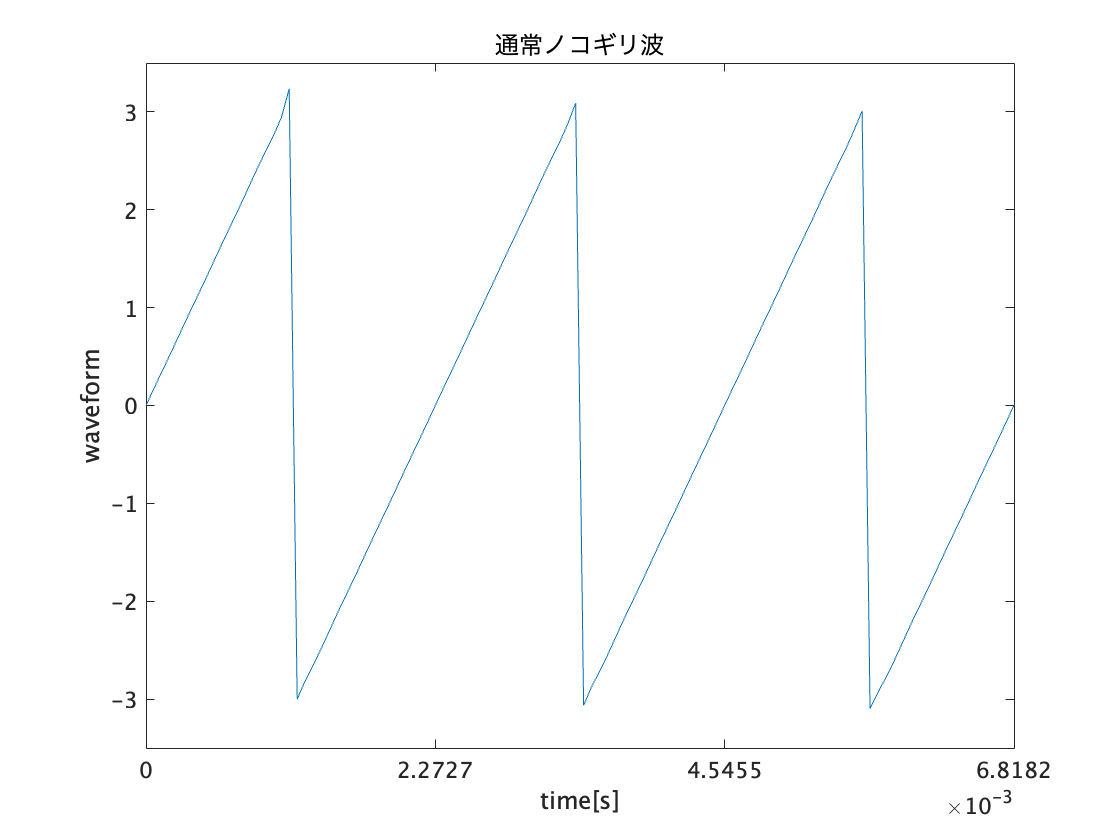
\includegraphics[keepaspectratio,width=0.85\textwidth]{nokogiri.png}
    \end{figure}
\end{frame}
\begin{frame}[t]{\showsec ノコギリ波}
    \begin{align}
        y(t) & =t             & (-\pi<t<\pi)     \\
        \intertext{を周期\(2\pi\)の関数として周期的に拡張したもの.}
        y(t) & = y(t + 2k\pi) & (k\in\mathbb{Z})
    \end{align}
    \begin{block}{ノコギリ波のフーリエ級数展開}
        \begin{align}
            y(t) & =\sum_{k=1}^{\infty}(-1)^{k-1}\dfrac{2}{k}\sin(kt)\label{nokogiri}
        \end{align}
    \end{block}
    \(\displaystyle\sum_{k=1}^{\infty}\)の\(\infty\)は今回,\texttt{50}としてプログラミングしている.
\end{frame}
\section{課題1}
\subsection{問題}
\begin{frame}[t,containsverbatim]{\showsec 課題1}
    \begin{exampleblock}{}
        矩形波・ノコギリ波を基本周波数を 440Hz 等の可聴域の範囲で作成し,さらに各周波数成分も位相を適当な値に変化させよう.\\
        (サンプリング周波数\verb|Fs = 16kHz|,長さ\verb|2s|.)
        \begin{itemize}
            \item 位相の操作
                  \begin{itemize}
                      \item 固定値 \(\pi/4\)
                      \item 固定値 \(\pi/2\)
                      \item ランダム値\footnote{ランダム値は \texttt{variable = rand} で格納できる.}
                  \end{itemize}
        \end{itemize}
    \end{exampleblock}
    \begin{block}{Tips}
        \begin{lstlisting}[language={Matlab},numbers={none},frame={none},xleftmargin=0em]
axis([xmin xmax ymin ymax]);
        \end{lstlisting}
        グラフをプロットするときの範囲を指定できる.周波数\(f\)の周期関数を\texttt{n}周期分プロットしたい場合は\texttt{xmin}を\texttt{0},\texttt{xmax}を\texttt{n/f}に設定する.
    \end{block}
\end{frame}
\subsection{サンプルコード}
\begin{frame}[t,containsverbatim]{\showsec 課題1(サンプルコード)}
    \begin{lstlisting}[language={Matlab}]
clear all;
Fs = 16000; % サンプリング周波数
f = 400;    % 基本周波数
t = [0 : ??] /Fs % 時間軸テーブル
phi1 = pi / 4;   % 初期位相 pi/2
phi2 = pi / 2;   % 初期位相 pi/4
phi3 = rand;     % 初期位相 ランダム
% --- ノコギリ波生成 ---
for k=1:50 % とりあえず50にでも設定しておく
    y1 = ?? + (-1)^(k-1) * 1/3 * 2/k * sin(??);
    y2 = ...;
    y3 = ...;
end
...
\end{lstlisting}
    \begin{block}{}
        \texttt{??}は,『何かしら入る』という意味なので,いろんなものが入る.(変数1つとは限らない)
    \end{block}
\end{frame}
\subsection{結果:ノコギリ波}
\begin{frame}{\showsec 課題1(結果:ノコギリ波)}
    \begin{figure}
        \centering
        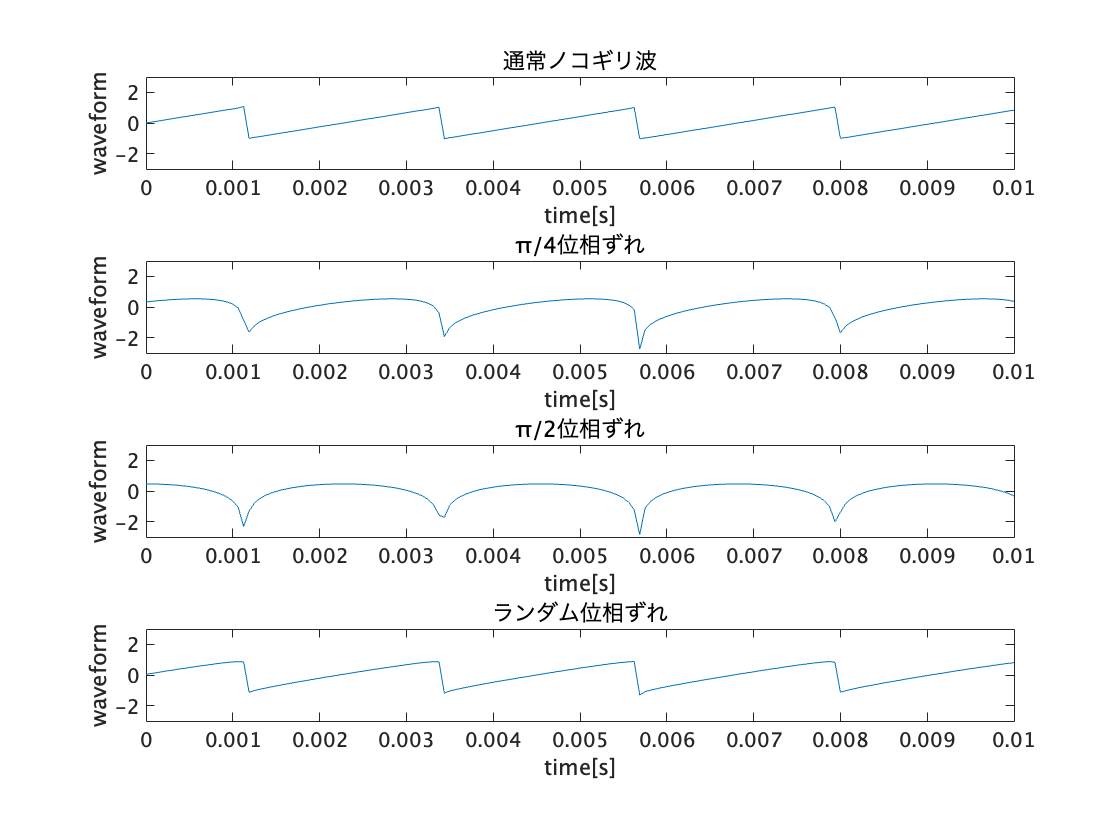
\includegraphics[keepaspectratio,width=0.89\textwidth]{no1_1_ans.png}
    \end{figure}
\end{frame}
\subsection{結果:矩形波}
\begin{frame}{\showsec 課題1(結果:矩形波)}
    \begin{figure}
        \centering
        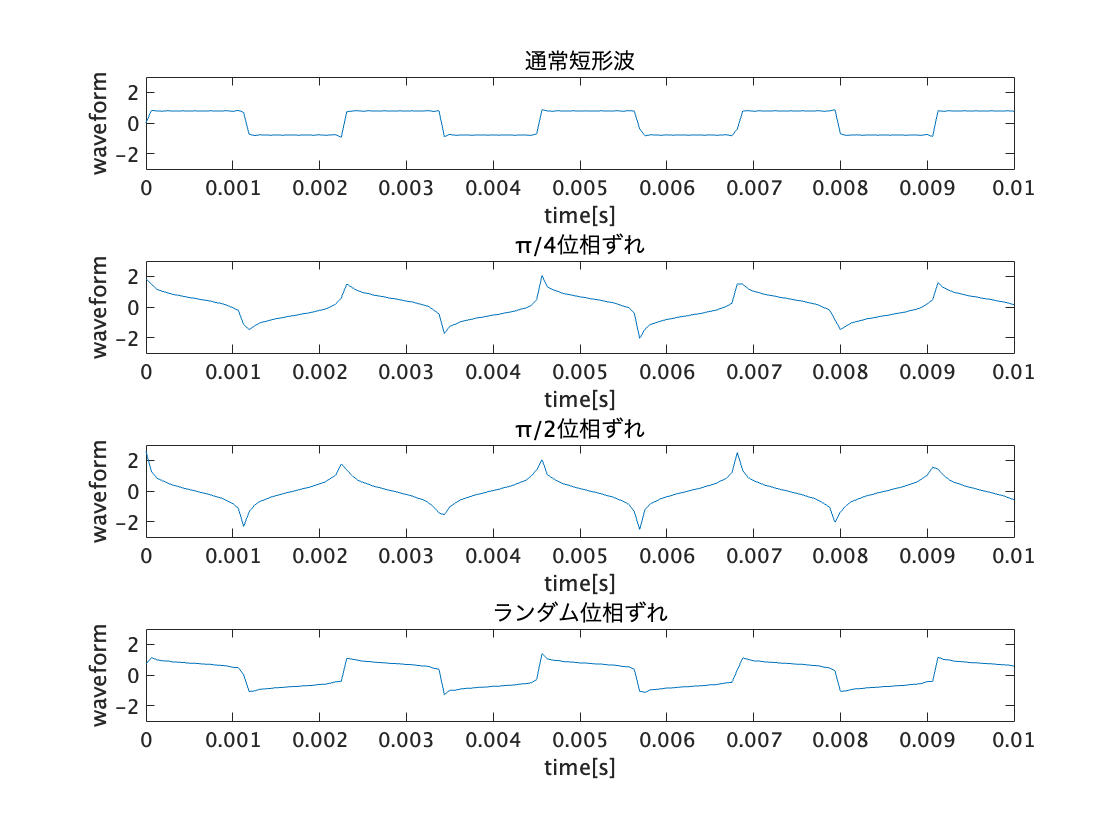
\includegraphics[keepaspectratio,width=0.89\textwidth]{no1_2_ans.png}
    \end{figure}
\end{frame}
\section{モノラルとステレオ}
\begin{frame}[t,containsverbatim]{\showsec モノラルとステレオ(\texttt{audioread})}
    \texttt{audioread}関数は,\texttt{filename.wav}のサンプルデータ\texttt{y}と,サンプリング周波数\texttt{Fs}を保存する関数である.
    \begin{lstlisting}[language={Matlab},xleftmargin={0mm},frame={lines}]
[y, Fs] = audioread('filename.wav');
\end{lstlisting}
    \begin{minipage}[t]{.49\textwidth}
        \begin{itemize}
            \item モノラルオーディオの場合\\
                  \texttt{y}は\texttt{N}行\texttt{1}列のデータ列
        \end{itemize}
    \end{minipage}
    \begin{minipage}[t]{.49\textwidth}
        \begin{itemize}
            \item ステレオオーディオの場合\\
                  \texttt{y}は\texttt{N}行\texttt{2}列のデータ列
        \end{itemize}
    \end{minipage}
    \vspace{2em}\\
    ステレオからモノラルに変換するには,\texttt{y}の2列目を削除すれば良い.
\end{frame}
\section{課題2}
\subsection{結果}
\begin{frame}[t]{\showsec 課題2}
    \begin{exampleblock}{}
        自分の母音の音声を4s程度ずつ録音し,その音声データの波形の上下を反転さよう.
        元データと反転後のデータを聴き比べよう.
    \end{exampleblock}
    \begin{figure}
        \centering
        \begin{minipage}[t]{0.49\textwidth}
            \centering
            \caption{それぞれのグラフ}
            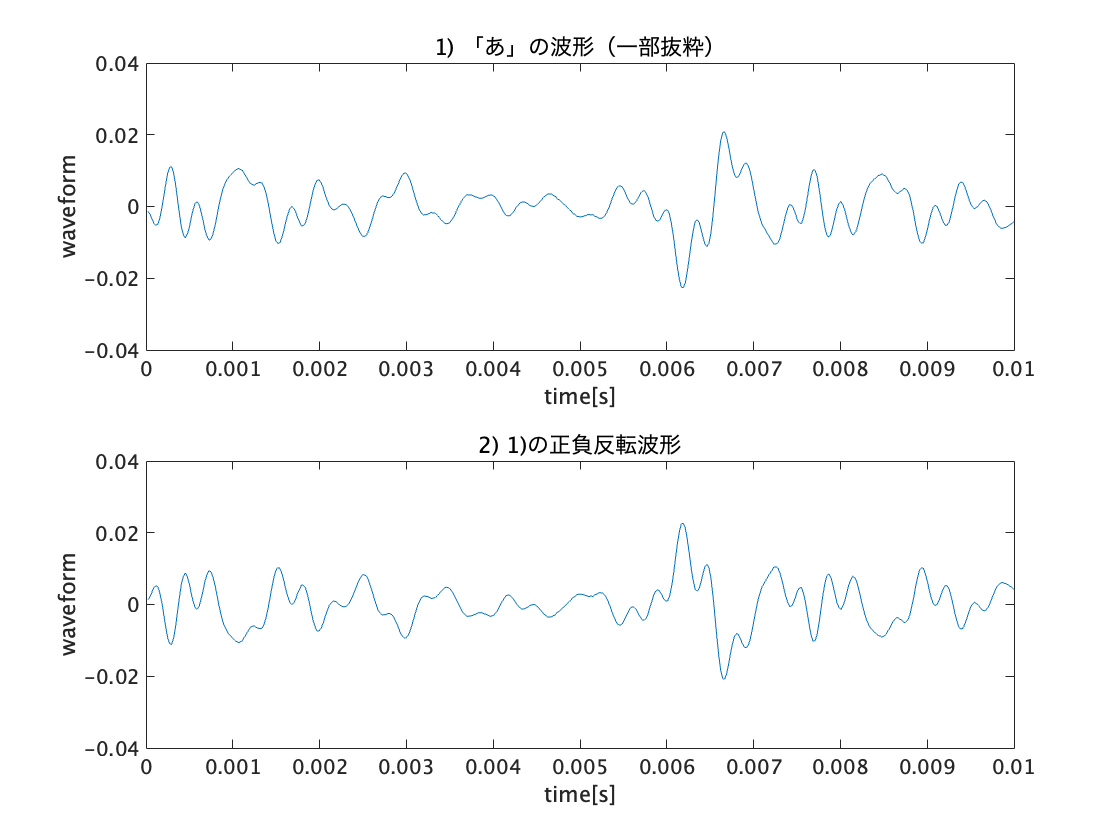
\includegraphics[keepaspectratio,width=\textwidth]{no2_ans_1.png}
        \end{minipage}
        \begin{minipage}[t]{0.49\textwidth}
            \centering
            \caption{グラフを重ね合わせてみる}
            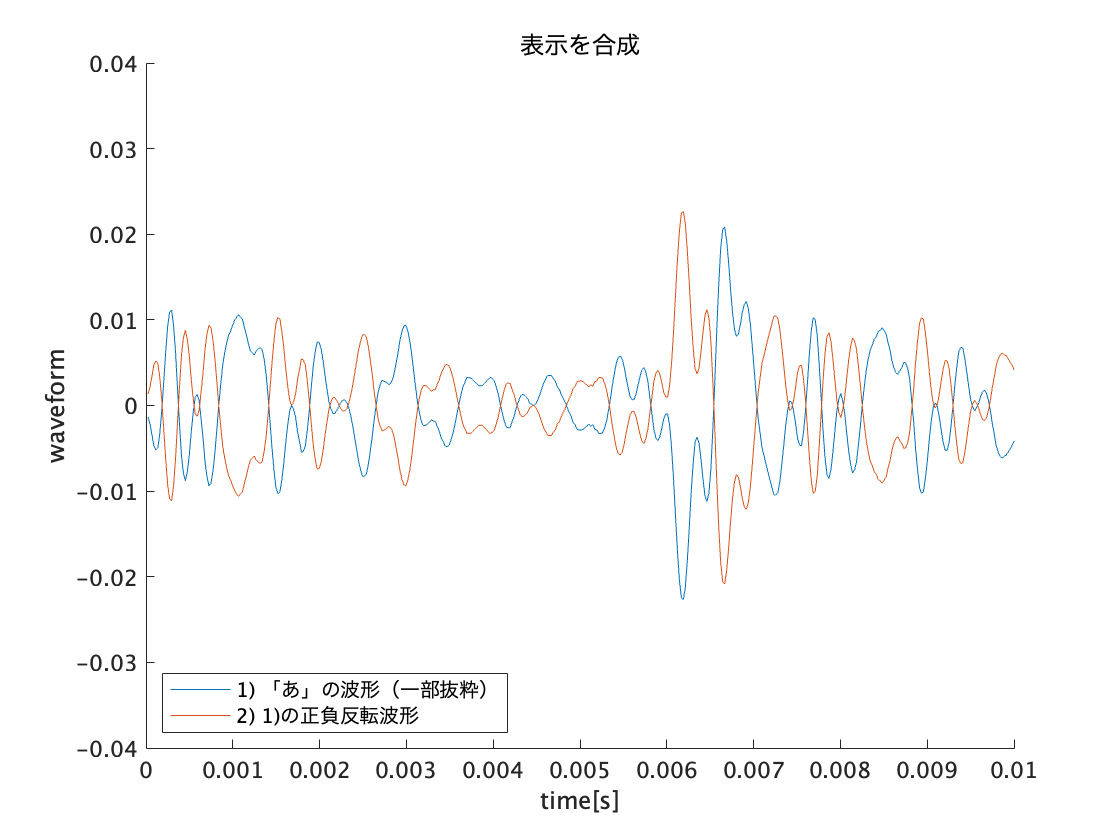
\includegraphics[keepaspectratio,width=\textwidth]{no2_ans_2.png}
        \end{minipage}
    \end{figure}
\end{frame}
\subsection{サンプルコード}
\begin{frame}[t,containsverbatim]{\showsec 課題2(サンプルコード)}
    \begin{lstlisting}[language={Matlab}]
clear;
[y, Fs] = audioread('sound1.wav');
y=?? % ステレオからモノラルへの変換
N = ??; % yの長さ
t = (1:??) /??; % 時間軸テーブル
z = ??; % yの各要素に対して正ならば負,負ならば正にする
...
    \end{lstlisting}
    \begin{alertblock}{}
        ステレオからモノラルへの変換をすること!
        \begin{itemize}
            \item 左右それぞれの信号が処理されグラフが見難くなったり
            \item そもそもデータ数が想定していたものと異なるので\texttt{plot}されなかったり
        \end{itemize}
    \end{alertblock}
\end{frame}
\addtocontents{toc}{\newpage}
\section{周波数解析}
\subsection{ノコギリ波}
\begin{frame}[t]{\showsec 周波数解析(ノコギリ波)}
    ノコギリ波は以下の式で表せる.
    \begin{align}
        y(t) & = \sum_{k=1}^{\infty}(-1)^{k-1}\dfrac{2}{k}\sin(kt)\tag{\ref{nokogiri}}    \\
             & = 2\sin(t) - \sin(2t) + \frac{2}{3}\sin(3t) - \frac{1}{2}\sin(4t) + \cdots
    \end{align}
    \begin{figure}
        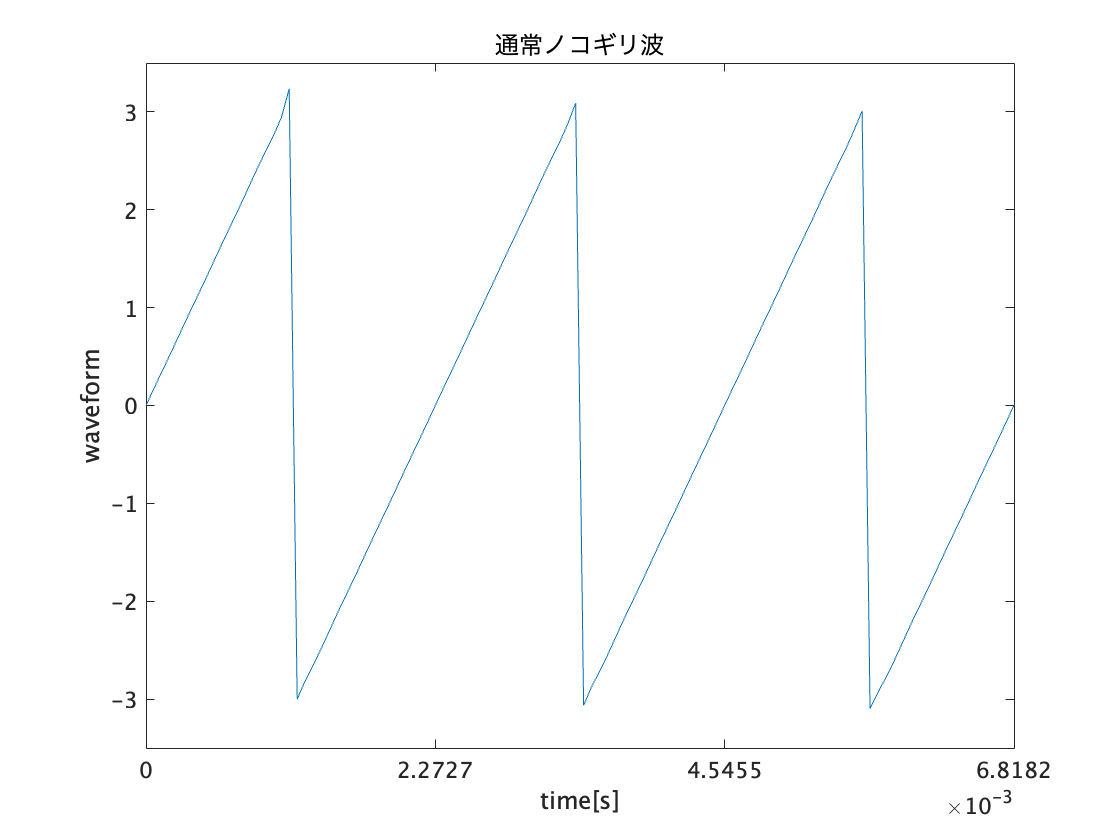
\includegraphics[keepaspectratio,height=0.5\textheight]{nokogiri.png}
    \end{figure}
\end{frame}
\subsection{振幅スペクトル}
\begin{frame}[t]{\showsec 周波数解析(振幅スペクトル)}
    \renewcommand{\arraystretch}{1.5}
    \begin{columns}
        \begin{column}[T]{0.44\textwidth}
            \begin{table}
                \begin{tabular}{r|cc}
                    \multicolumn{1}{c}{正弦波}   & 振幅                                                            & 周波数                                                             \\
                    \hline
                    \(2\sin(t)\)              & \tikz[remember picture,baseline=(A.base)]{\node(A){\(2\)}}    & \tikz[remember picture,baseline=(D.base)]{\node(D){\(1/2\pi\)}} \\
                    \(-\sin (2t)\)            & \(-1\)                                                        & \(1/\pi\)                                                       \\
                    \(\frac{2}{3}\sin (3t)\)  & \(2/3\)                                                       & \(3/2\pi\)                                                      \\
                    \(-\frac{1}{2}\sin (4t)\) & \tikz[remember picture,baseline=(C.base)]{\node(C){\(-1/2\)}} & \tikz[remember picture,baseline=(B.base)]{\node(B){\(2/\pi\)}}  \\
                    \multicolumn{3}{c}{{\LARGE\vdots}}
                \end{tabular}
            \end{table}
            \begin{tikzpicture}[remember picture,overlay]
                \node[inner sep=0.1mm,fit={(A)(B)(C)(D)},draw,rounded corners,draw=blue](warp){};
            \end{tikzpicture}
            \begin{align*}
                (-1)^{k-1}\dfrac{2}{k}\sin(kt) &  & (k\in\mathbb{N})
            \end{align*}
        \end{column}
        \begin{column}[T]{0.55\textwidth}
            \begin{figure}
                \caption{振幅スペクトル}
                \vspace{-1em}
                \begin{tikzpicture}[remember picture]
                    \node[left] at(0,0){O};
                    \draw[very thick,-Stealth](0,0)--(5,0)node[midway,fill=white]{\scriptsize 周波数};
                    \draw[very thick,-Stealth](0,-1.6)--(0,4.1)node[left]at($(0,0)!0.5!(0,4.1)$){\scriptsize \rotatebox{90}{振幅}};
                    \foreach \u \v in {0.4/3,0.8/-1.5,1.2/1,1.6/-0.75}
                    \draw[thick,blue](\u,0)--(\u,\v);
                    \foreach \u \v \z in {0.4/{\(1/2\pi\)}/below,0.8/{\(1/\pi\)}/above,1.2/{\(3/2\pi\)}/below,1.6/{\(2/\pi\)}/above}
                    \node[\z] at(\u,0){\tiny\v};
                    \coordinate (O) at (0,0);
                    \foreach \u \v \z \w in {0.4/3/a/{\(2\)},0.8/-1.5/b/{\(-1\)},1.2/1/c/{\(2/3\)},1.6/-0.75/d/{\(-1/2\)}} {
                    \coordinate (\z) at (\u,\v);
                    \draw[dotted,thin](\z)--(O |- \z)node[left]{\tiny\w};
                    }
                \end{tikzpicture}
                \begin{tikzpicture}[remember picture,overlay]
                    \draw[-latex,very thick,dashed]($(warp.south east)!0.5!(warp.south west)$)to[bend right=30]($(O)+(-0.5cm,0)$);
                \end{tikzpicture}
            \end{figure}
        \end{column}
    \end{columns}
\end{frame}
\subsection{\texttt{fft}}
\begin{frame}[t,containsverbatim]{\showsec 周波数解析(\texttt{fft})}\label{frame:fft}
    \begin{lstlisting}[language={Matlab},frame={lines},numbers={none},xleftmargin={0mm}]
fft_y = fft(y); % データ列yに対してfft を行う.
                    \end{lstlisting}
    \begin{block}{}
        \texttt{fft}は,データ列\texttt{y}を高速フーリエ変換する関数であるが,入力データ列\texttt{y}に対して出力データ列\texttt{fft(y)}のデータ長は,入力データ列\texttt{y}と一致する.\\
        ただし,indexとその内容についてはそれぞれ異なる.
        \begin{itemize}
            \item 入力データ列\texttt{y}のindexは時刻に対応.\footnotemark[1]
            \item 出力データ列\texttt{fft(y)}のindexは周波数に対応.\footnotemark[2]
        \end{itemize}
        \footnotetext{\footnotemark[1]\footnotemark[2]indexが時刻や周波数というわけではない.}
    \end{block}
\end{frame}
\subsection{\texttt{fftshift}}
\begin{frame}[t,containsverbatim]{\showsec 周波数解析(\texttt{fftshift})}
    \begin{itemize}
        \item サンプリング周波数\texttt{Fs}の信号\texttt{y}に対して高速フーリエ変換\texttt{fft}を行うだけでは周波数解析ができない!\\
        \item \texttt{fft}では\(\textrm{\texttt{-Fs/2}}\leq \textrm{周波数成分}\leq\textrm{\texttt{Fs/2}}\)を得られる.
        \item ただし,正のデータ・負のデータが(左右)が入れ替わった状態で出力される.
    \end{itemize}
    \begin{figure}
        \centering
        \begin{minipage}[t]{0.49\textwidth}
            \centering
            \caption{\texttt{fft}を行った直後(\texttt{ftt\_y})}
            \label{fig:fft}
            \begin{tikzpicture}
                \draw[thick](0,0)--(0.9\textwidth,0)--(0.9\textwidth,0.5)--(0,0.5)--cycle;
                \node[below] at (0,0)(a){\tiny\texttt{1}};
                \node[above right] at (0,0.5){\tiny\texttt{0}};
                \node[above left] at ($(.9\textwidth,0.5)!0.5!(0,0.5)$){\tiny\texttt{Fs/2}};
                \node[above right] at ($(.9\textwidth,0.5)!0.5!(0,0.5)$){\tiny\texttt{-Fs/2}};
                \node[above left] at (.9\textwidth,0.5){\tiny\texttt{-1/Fs}};
                \node[below] at (0.9\textwidth,0)(b){\tiny\texttt{Fs}};
                \draw[latex-latex](a)--(b)node[midway,below]{\tiny\texttt{index}};
                \coordinate (C) at ($(0.9\textwidth,0)!0.5!(0,0)$);
                \draw[thick](C)--($(C)+(0,1.5mm)$);
                \coordinate (c) at ($(0.9\textwidth,0.5)!0.5!(0,0.5)$);
                \draw[thick](c)--($(c)+(0,-1.5mm)$);
                \node at($(C)!0.5!(0,5mm)$){\tiny 正のデータ};
                \node at($(c)!0.5!(0.9\textwidth,0mm)$){\tiny 負のデータ};
            \end{tikzpicture}
        \end{minipage}
        \begin{minipage}[t]{0.49\textwidth}
            \centering
            \caption{理想的な状態}
            \label{fig:fftshift}
            \begin{tikzpicture}
                \draw[thick](0,0)--(0.9\textwidth,0)--(0.9\textwidth,0.5)--(0,0.5)--cycle;
                \node[below] at (0,0)(a){\tiny\texttt{1}};
                \node[above right] at (0,0.5){\tiny\texttt{-Fs/2}};
                \node[above left] at ($(.9\textwidth,0.5)!0.5!(0,0.5)$){\tiny\texttt{-1/Fs}};
                \node[above right] at ($(.9\textwidth,0.5)!0.5!(0,0.5)$){\tiny\texttt{0}};
                \node[above left] at (.9\textwidth,0.5){\tiny\texttt{Fs/2}};
                \node[below] at (0.9\textwidth,0)(b){\tiny\texttt{Fs}};
                \draw[latex-latex](a)--(b)node[midway,below]{\tiny\texttt{index}};
                \coordinate (C) at ($(0.9\textwidth,0)!0.5!(0,0)$);
                \draw[thick](C)--($(C)+(0,1.5mm)$);
                \coordinate (c) at ($(0.9\textwidth,0.5)!0.5!(0,0.5)$);
                \draw[thick](c)--($(c)+(0,-1.5mm)$);
                \node at($(C)!0.5!(0,5mm)$){\tiny 負のデータ};
                \node at($(c)!0.5!(0.9\textwidth,0mm)$){\tiny 正のデータ};
            \end{tikzpicture}
        \end{minipage}
    \end{figure}
\end{frame}
\begin{frame}[t,containsverbatim]{\showsec 周波数解析(\texttt{fftshift})}
    \begin{itemize}
        \item 図\ref{fig:fft},\ref{fig:fft_f}から図\ref{fig:fftshift},\ref{fig:fft_shift_f}の状態にするために\texttt{fftshift}関数を用いる.\\
              \begin{lstlisting}[language={Matlab},frame={lines},numbers={none},xleftmargin={0mm}]
fftshift_y = fftshift(fft_y);
            \end{lstlisting}
    \end{itemize}
    \begin{figure}
        \centering
        \begin{minipage}[t]{.49\textwidth}
            \centering
            \caption{\texttt{fft}}
            \label{fig:fft_f}
            \begin{tikzpicture}
                \node(fig){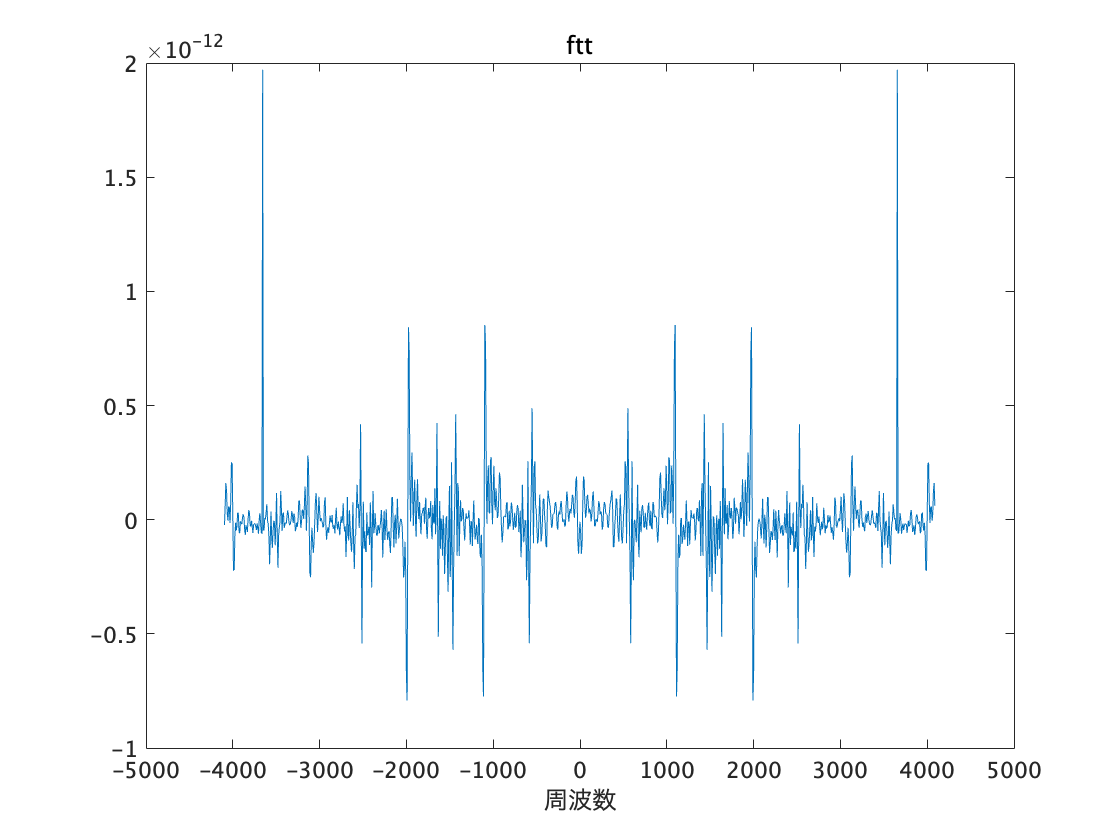
\includegraphics[keepaspectratio,width=.9\textwidth]{fft_fft.png}};
                \coordinate (figsouth) at (fig.south);
                \coordinate (figscenter) at ($(figsouth)+(0.98mm,5.7mm)$);
                \coordinate (figncenter) at ($(figscenter)+(0,3.24cm)$);
                \coordinate (figsleft) at ($(figscenter)+(-2.05cm,0)$);
                \coordinate (figsright) at ($(figscenter)+(2.05cm,0)$);
                % \draw[fill=black](figncenter)circle[radius=0.01];
                % \draw[fill=black](figscenter)circle[radius=0.01];
                % \draw[fill=black](figsleft)circle[radius=0.01];
                % \draw[fill=black](figsright)circle[radius=0.01];
                \fill[fill=red,opacity=0.1](figsleft)--(figsleft |- figncenter)--(figncenter)--(figscenter)--cycle;
                \fill[fill=blue,opacity=0.1](figsright)--(figsright |- figncenter)--(figncenter)--(figscenter)--cycle;
            \end{tikzpicture}
        \end{minipage}
        \begin{minipage}[t]{.49\textwidth}
            \centering
            \caption{\texttt{fftshift}}
            \label{fig:fft_shift_f}
            \begin{tikzpicture}
                \node(fig){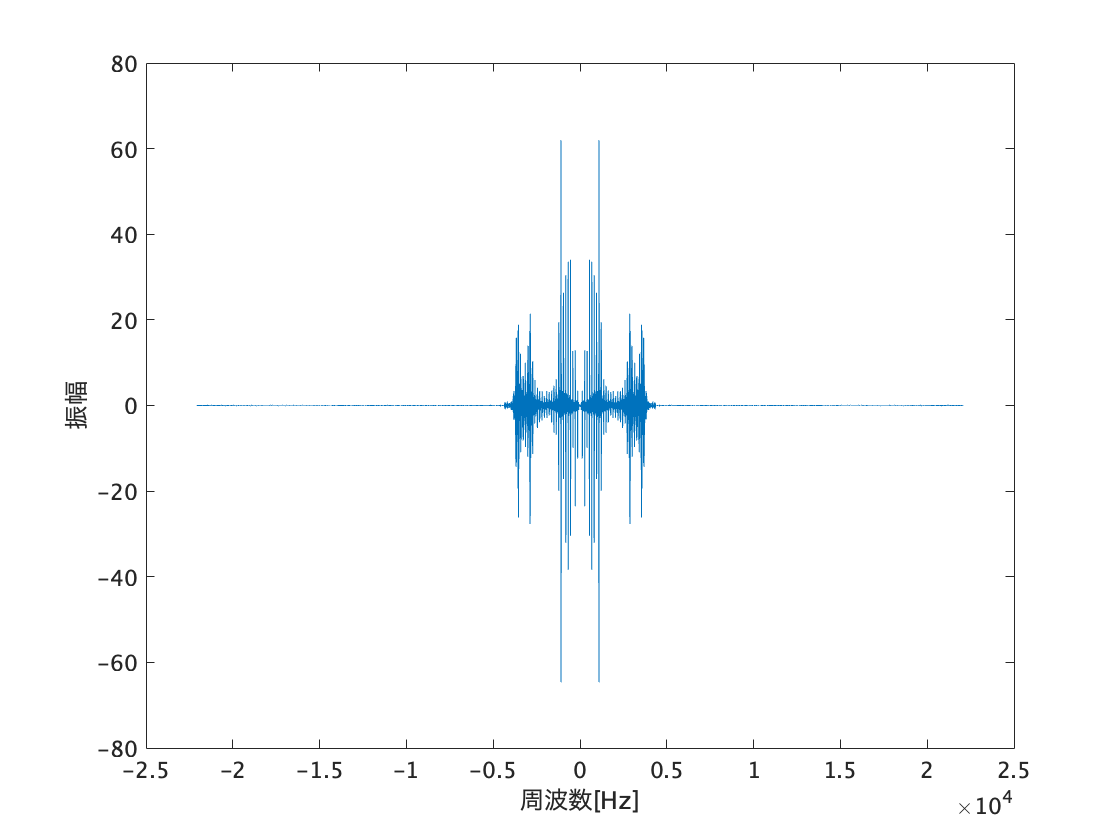
\includegraphics[keepaspectratio,width=.9\textwidth]{fft_fftshift.png}};
                \coordinate (figsouth) at (fig.south);
                \coordinate (figscenter) at ($(figsouth)+(0.98mm,5.7mm)$);
                \coordinate (figncenter) at ($(figscenter)+(0,3.24cm)$);
                \coordinate (figsleft) at ($(figscenter)+(-2.05cm,0)$);
                \coordinate (figsright) at ($(figscenter)+(2.05cm,0)$);
                \fill[fill=blue,opacity=0.1](figsleft)--(figsleft |- figncenter)--(figncenter)--(figscenter)--cycle;
                \fill[fill=red,opacity=0.1](figsright)--(figsright |- figncenter)--(figncenter)--(figscenter)--cycle;
            \end{tikzpicture}
        \end{minipage}
    \end{figure}
\end{frame}
\subsection{\texttt{abs}}
\begin{frame}[t,containsverbatim]{\showsec 周波数解析(\texttt{abs})}
    \begin{itemize}
        \item 絶対値を取るために\texttt{abs}をとる.\\
              \begin{lstlisting}[language={Matlab},frame={lines},numbers={none},xleftmargin={0mm}]
fftshift_abs_y = abs(fftshift_y);
                        \end{lstlisting}
    \end{itemize}
    \begin{figure}
        \centering
        \begin{minipage}{.49\textwidth}
            \centering
            \caption{\texttt{fftshift}}
            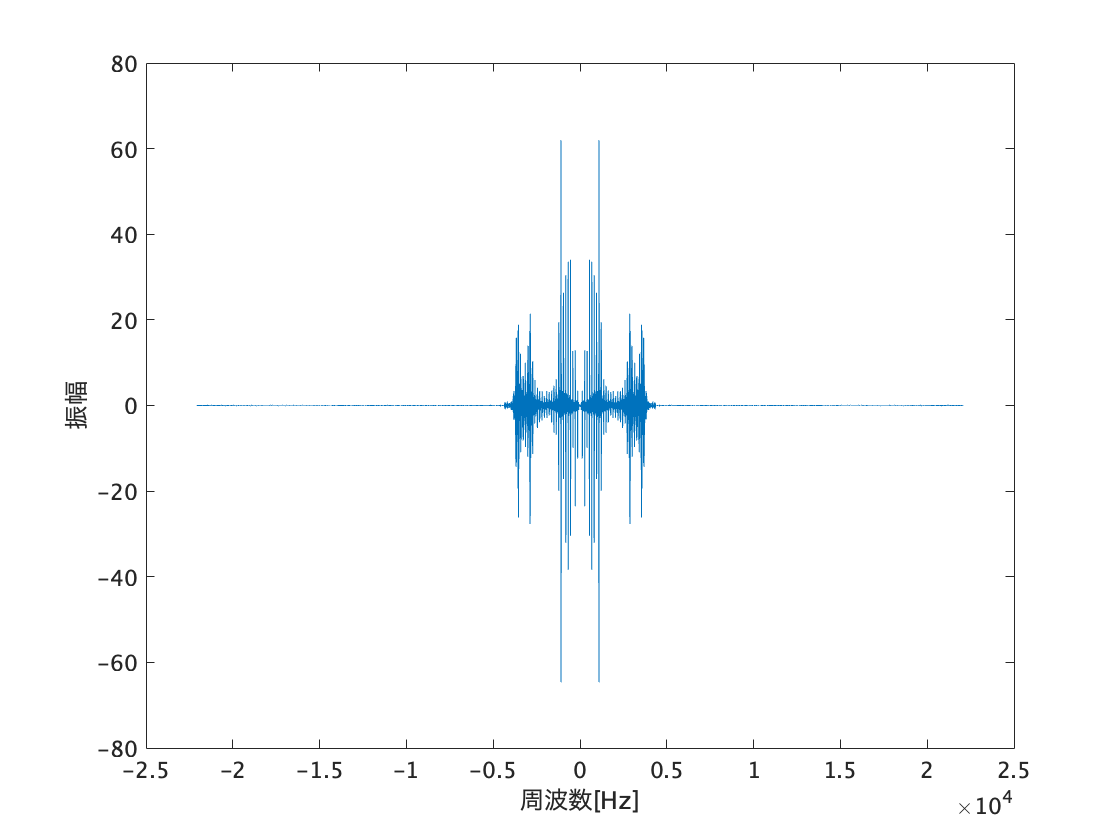
\includegraphics[keepaspectratio,width=\textwidth]{fft_fftshift.png}
        \end{minipage}
        \begin{minipage}{.49\textwidth}
            \centering
            \caption{\texttt{abs}}
            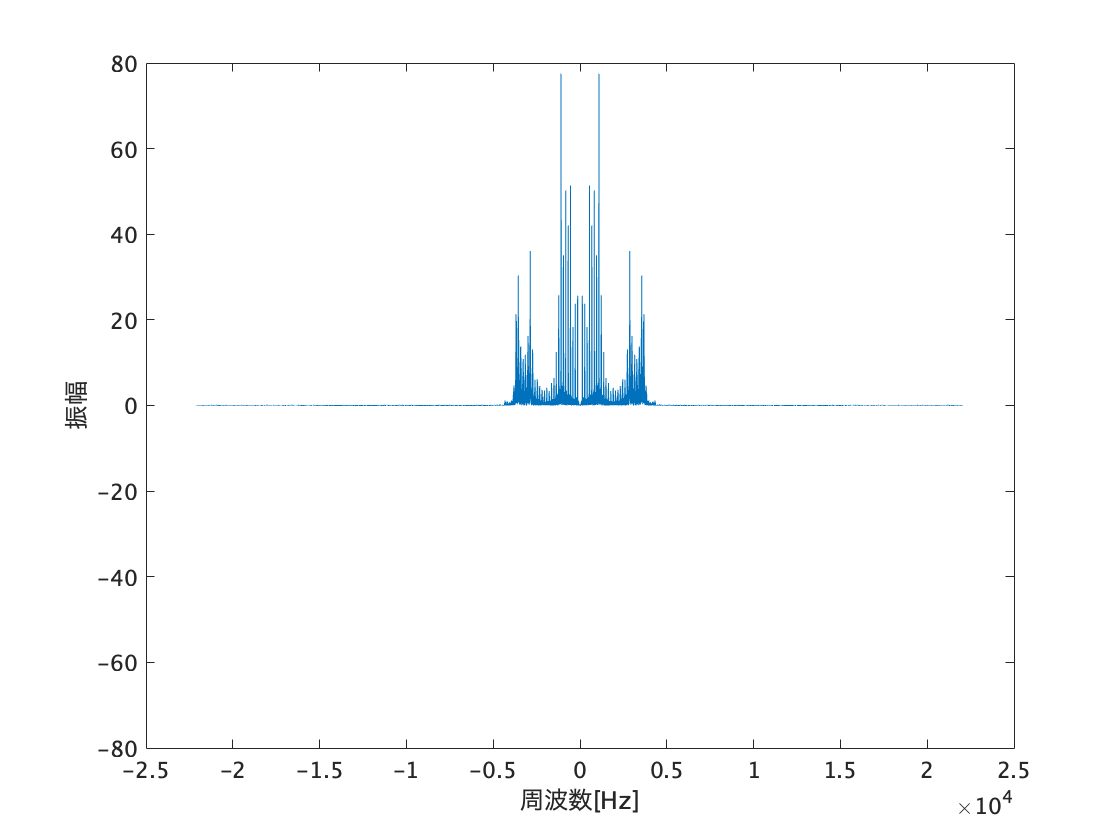
\includegraphics[keepaspectratio,width=\textwidth]{fft_abs.png}
        \end{minipage}
    \end{figure}
\end{frame}
\subsection{周波数テーブルの作成}
\begin{frame}[t,containsverbatim]{\showsec 周波数解析(周波数テーブルの作成)}
    これまでの工程で,\texttt{0}を中心として,正負にナイキスト周波数(\texttt{Fs/2})分離れた振幅データを得られる.
    \begin{enumerate}
        \item データの長さ\texttt{ln = length(abs(fftshift(fft(y))))}を取得する.\\\textcolor{gray}{(\texttt{length(fft(y)) = length(y),ln = length(y)}となる)→p.\pageref{frame:fft}}
        \item[?\ ] \textcolor{red}{10個のリンゴ}を\textcolor{blue}{5つの箱}へ均等に入れます.1箱あたり\(10/5\)個のリンゴが入っていますね.
        \item \textcolor{red}{データ長\texttt{ln}のデータ}を,\textcolor{blue}{サンプリング周波数\texttt{Fs}長の行列}に対応させるためには?
    \end{enumerate}
    \begin{figure}
        \centering
        \begin{tikzpicture}[remember picture]
            \node[above] at ($(0,0.5cm)!0.5!(10cm,0.5cm)$){\footnotesize\texttt{abs(fftshift(fft(y)))}で得られたデータ};
            \draw[thick](0,0)rectangle(10cm,0.5cm);
            \node at ($(0,0.5cm)!0.5!(0.5cm,0)$) {\tiny\texttt{1}};
            \node at ($(9.5cm,0.5cm)!0.5!(10cm,0)$) {\tiny\texttt{ln}};
            \foreach \u in {0.5,1,...,9.5}{
                    \draw(\u cm,0.5cm)--(\u cm,0.35cm);
                    \draw(\u cm,0cm)--(\u cm,0.15cm);}
            % \node at (0,-0.5cm){};
        \end{tikzpicture}
        \begin{tikzpicture}[remember picture]
            \node[above] at ($(0,0.5cm)!0.5!(10cm,0.5cm)$){\footnotesize 作りたい行列 \texttt{ = freq}};
            \draw[thick](0,0)rectangle(10cm,0.5cm);
            \node at ($(0,0.5cm)!0.5!(1cm,0)$) {\tiny\texttt{-Fs/2}};
            \node at ($(9cm,0.5cm)!0.5!(10cm,0)$) {\tiny\texttt{Fs/2}};
            \foreach \u in {1,2,...,9}{
                    \draw(\u cm,0.5cm)--(\u cm,0.35cm);
                    \draw(\u cm,0cm)--(\u cm,0.15cm);}
            \draw[latex-latex](0,-0.3cm)--(10cm,-0.3cm)node[midway,fill=white]{\tiny 長さ\texttt{Fs}};
        \end{tikzpicture}
    \end{figure}
    \begin{lstlisting}[language=Matlab,xleftmargin={0mm},frame={lines}]
freq = [-Fs/2 : ln/Fs : Fs/2 - ln/Fs];
    \end{lstlisting}
\end{frame}
\begin{frame}[t,containsverbatim]{\showsec 周波数解析(周波数テーブルの作成)}
    \begin{lstlisting}[language={Matlab},frame={lines},xleftmargin={0mm}]
plot(周波数テーブル, 振幅データ);
    \end{lstlisting}
    \begin{figure}
        \centering
        \begin{tikzpicture}
            \draw[very thick](0,0)node[below]{\texttt{-Fs/2}}--(10cm,0)node[midway,below]{\texttt{0}}node[below]{\texttt{Fs/2}};
            \draw[very thick](0,0)--(0,3cm)node[midway,left]{\rotatebox{90}{振幅}};
            \draw[very thick,dashed](0,3cm)--(0,4cm);
            \node[left] at (0,0){\texttt{0}};
            \node at (5cm,-0.7cm){周波数};
            \fill[gray!10] ($(0,0)!0.5!(10cm,4cm)$) circle (4.9cm and 1.9cm)node[black]{データ\texttt{y}の振幅スペクトル};
        \end{tikzpicture}
    \end{figure}
\end{frame}
\section{課題3}
\begin{frame}[t]{\showsec 課題3}
    \begin{exampleblock}{}
        \begin{enumerate}
            \item 課題2で録音した各音声を周波数解析し,スペクトル上でピークのある周波数およびその周波数のY軸の値を抽出しよう.
            \item 抽出した周波数,Y軸の値の順音を合成し,音の違いを聴き比べる.
        \end{enumerate}
    \end{exampleblock}
    \dotfill
    \begin{itemize}
        \item 0Hz - 10,000Hz 程度までの範囲で,ピークとなる周波数,及びそのピーク値を高い順から10個程度以上抽出する.\\
              \begin{itemize}
                  \item とりあえず,手動で10個抽出する.
              \end{itemize}
        \item 周波数およびピーク値(Y軸の値)は厳密でなくて良い.
        \item \texttt{a},\texttt{i}の合成音の聞こえ方の違い,及び元の音声との違いについて考察する.
    \end{itemize}
\end{frame}
\subsection{サンプルコード:解析}
\begin{frame}[t,containsverbatim]{\showsec 課題3(サンプルコード:解析)}
    \begin{lstlisting}[language=Matlab]
clear;
% --- "a" の音声 ---
[y_a, Fs_a] = audioread('sound_a.wav');
y_a = y_a(??); % ステレオからモノラルへの変換
t_a = [0 : length(??)-??]/ ??; % 時間軸テーブル
Y_a  = ??; % 高速フーリエ変換
YS_a = ??; % fftshift
YS_a_abs = ??; % 絶対値を取る
YS_a_len = length(YS_a_abs); % YS_a_absのデータ長を取得

% 周波数テーブル作成
freq_a = [-Fs_a/2 : ?? : Fs_a/2 - ??];

figure;
plot(??, ??); % 一度グラフにplotしてみる
axis([0 5000 0 80]); % 0Hz - 5000Hz まで表示する
\end{lstlisting}
\end{frame}
\begin{frame}[t,containsverbatim]{\showsec 課題3(サンプルコード:解析)}
    \begin{figure}
        \centering
        \begin{minipage}{0.48\textwidth}
            \centering
            \caption{振幅スペクトル}
            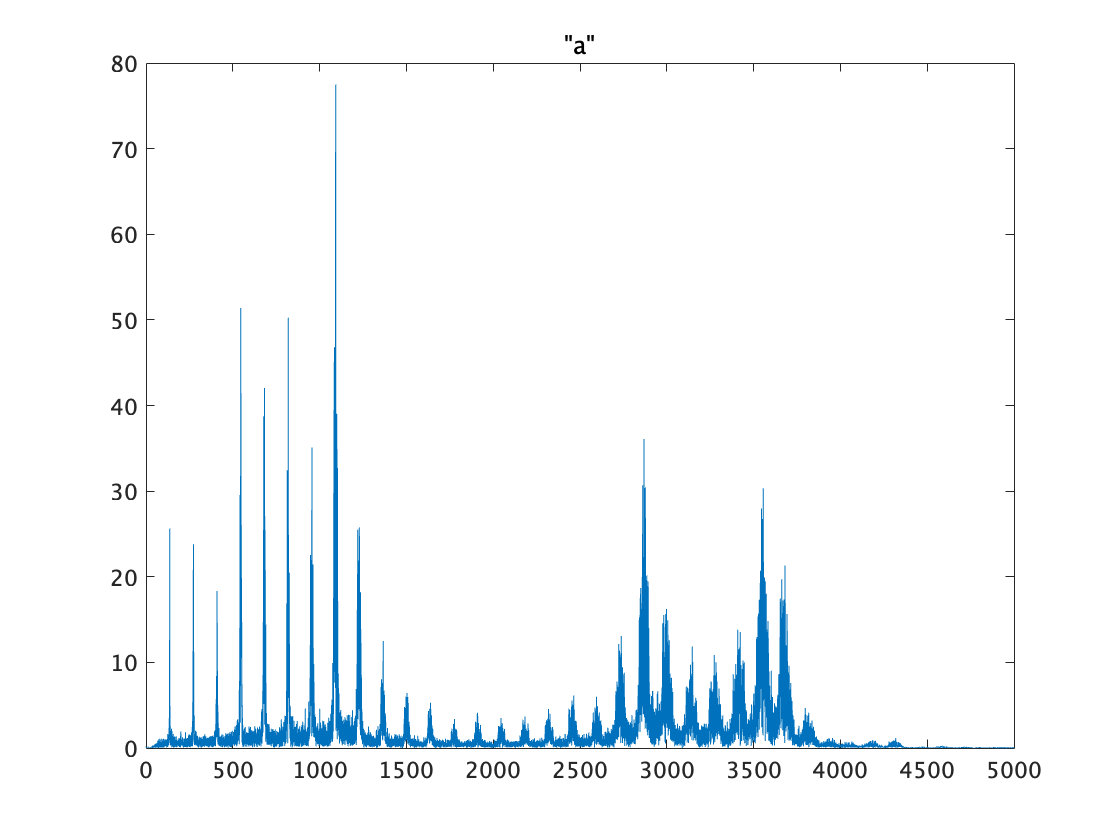
\includegraphics[keepaspectratio,width=\textwidth]{freq.png}
        \end{minipage}
        \begin{minipage}{0.48\textwidth}
            \centering
            \caption{振幅が大きいところ10点選ぶ}
            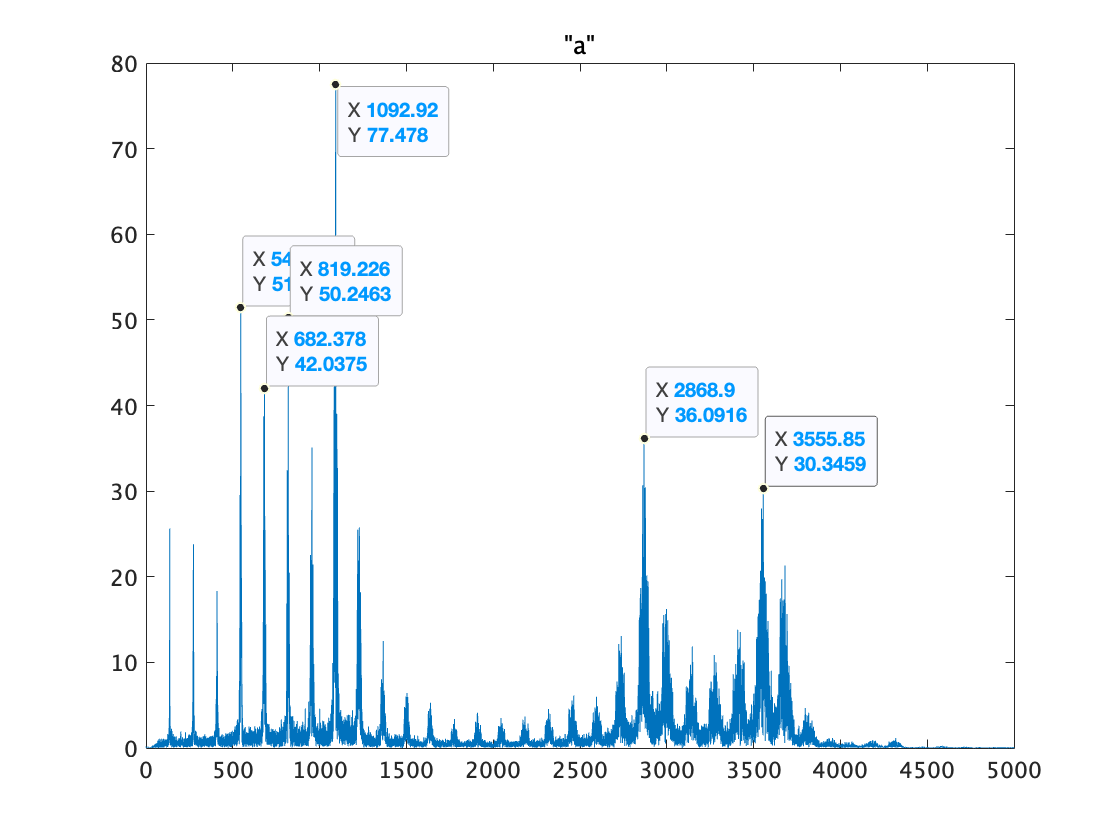
\includegraphics[keepaspectratio,width=\textwidth]{pointselect.png}
        \end{minipage}
    \end{figure}
    \begin{itemize}
        \item plotした点を行列に記す.
    \end{itemize}
    \begin{lstlisting}[language={Matlab},firstnumber={last}]
a_x = [1093 2867 ... 682]
a_y = [77 36 ...  ... 42]
    \end{lstlisting}
\end{frame}
\subsection{サンプルコード:合成}
\begin{frame}[t,containsverbatim]{\showsec 課題3(サンプルコード:合成)}
    \begin{lstlisting}[language={Matlab},firstnumber={last}]
ya = 0;
for k=1:10  % t_a は時間軸テーブル
    ya = ?? + ?? * sin(2*pi* ?? *t_a);
end
\end{lstlisting}
    \begin{minipage}[t]{0.48\textwidth}
        \centering
        \begin{figure}
            \centering
            \caption{\scriptsize\texttt{y\_a}を\texttt{t\_a}に対してプロットした結果}
            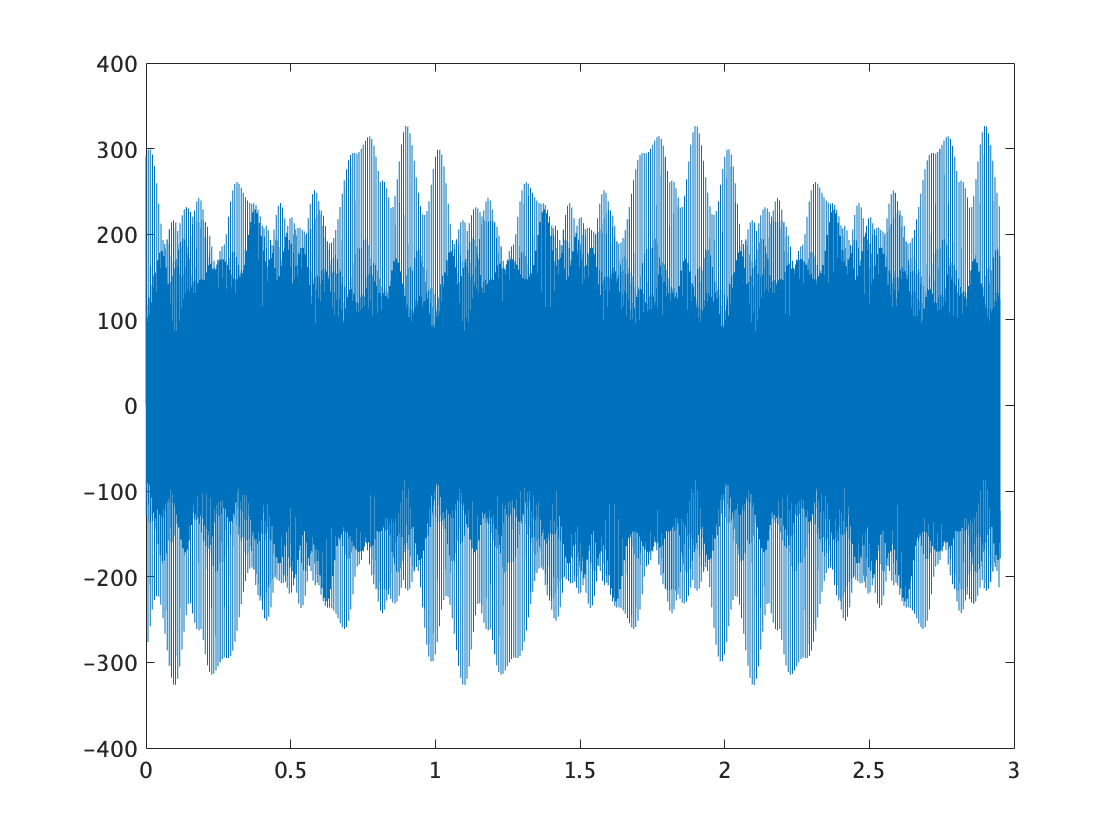
\includegraphics[keepaspectratio,height=.45\textheight]{no3.png}
        \end{figure}
    \end{minipage}
    \begin{minipage}[t]{0.48\textwidth}
        \begin{itemize}
            \item \texttt{a\_x}は周波数,\texttt{a\_y}は振幅であることを思い出す.
            \item それらの重ね合わせで音が再現されていたことを思い出す.\\(フーリエ級数展開)
            \item 周波数\(f\)の正弦波は\[y(t)=\sin(2\pi ft)\]であることを思い出す.
        \end{itemize}
    \end{minipage}
\end{frame}
\end{document}